%!TEX root = ../main.tex
\chapter{Experimentos e Resultados}

\begin{table}[ht]
\begin{center}
\begin{tabular}{c|ccccc}
Material & Densidade ($\nicefrac{kg}{m^3}$) & Módulo de Young (GPa) & Razão de Poisson & $\alpha$ & $\beta$\\
\hline Cerâmica & $2700$ & $7.4 \times 10^{10}$ & $0.19$ & $6$ & $1 \times 10^{-7}$\\
Aço & $1050$ & $3.5 \times 10^9$ & $0.34$ & $30$ & $8 \times 10^{-7}$\\
\end{tabular}
\end{center}
\caption{Parâmetros de Materiais}\label{tab:material_parameters}
\end{table}

\section{Benchmark}
Before the Titan, computing all 6 fields for the Acceleration Noise in a $176^3$ grid would take ~110ms. After installing the Titan card, it is taking ~12ms (I didn't even recompiled the code). Now I can use the profiler and hopefully I will be able to reduce that by another factor.

15 segundos por modo


\section{Teste Numérico}

Para testarmos numericamente o nosso método

Para testarmos numericamente o nosso método

Para testarmos numericamente o nosso método

Para testarmos numericamente o nosso método

\begin{figure}[ht]
\centering
\begin{subfigure}{0.6\textwidth}
	\centering
	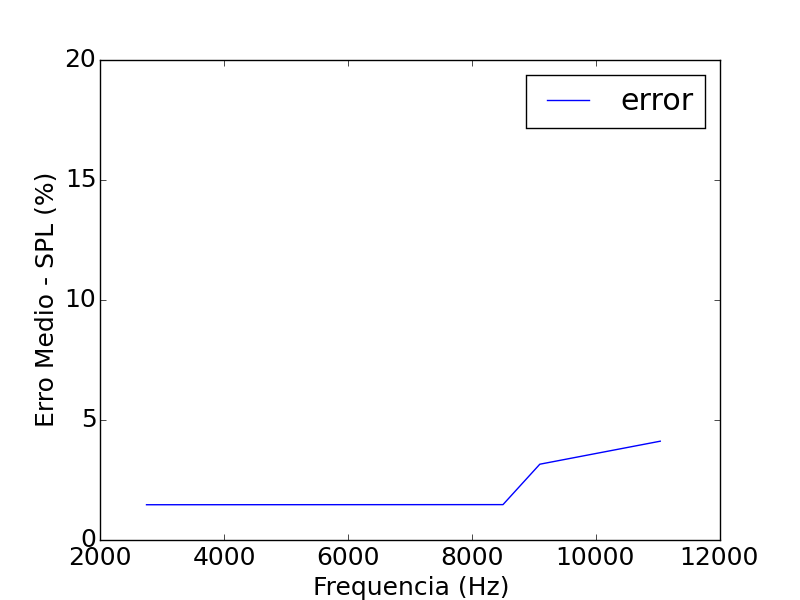
\includegraphics[width=\textwidth]{../data/transfer_test/steel_key/plots/steel_key_error.png}
	\caption{}\label{fig:coef_key_err}
\end{subfigure}
\begin{subfigure}{0.5\textwidth}
	\centering
	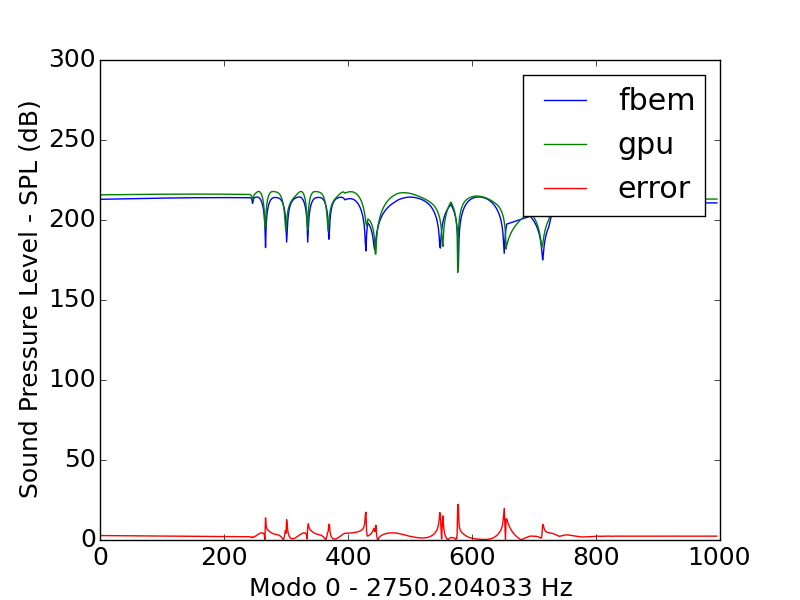
\includegraphics[width=\textwidth]{../data/transfer_test/steel_key/plots/steel_key-tfv-0_0.png}
	\label{fig:coef_key_0}
\end{subfigure}%
\begin{subfigure}{0.5\textwidth}
	\centering
	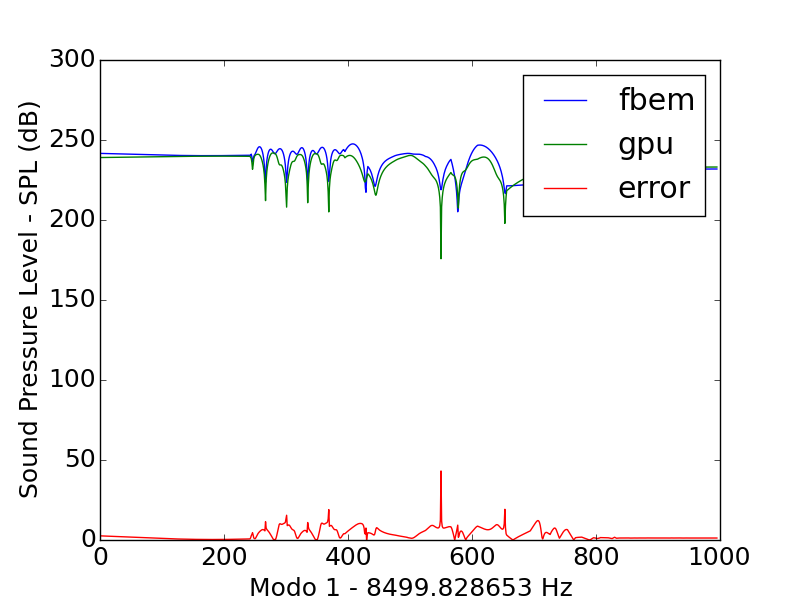
\includegraphics[width=\textwidth]{../data/transfer_test/steel_key/plots/steel_key-tfv-0_1.png}
	\label{fig:coef_key_1}
\end{subfigure}
\begin{subfigure}{0.5\textwidth}
	\centering
	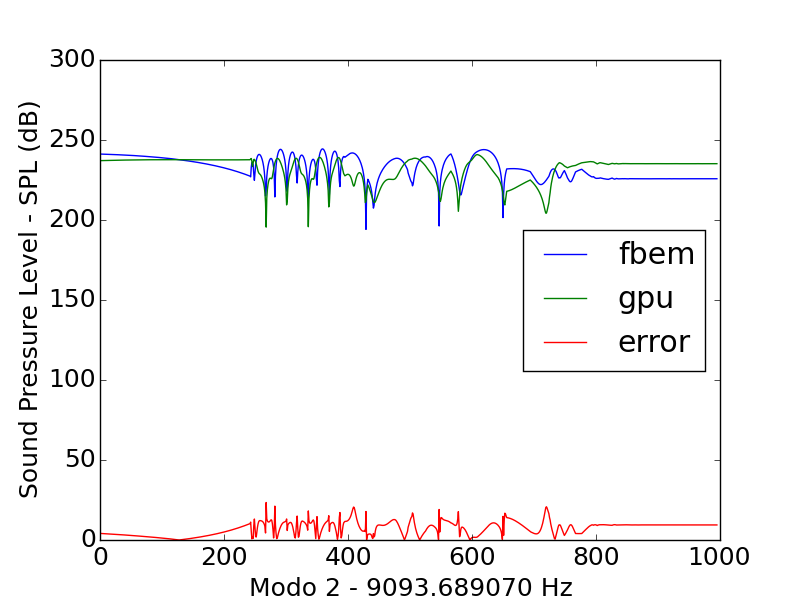
\includegraphics[width=\textwidth]{../data/transfer_test/steel_key/plots/steel_key-tfv-0_2.png}
	\label{fig:coef_key_2}
\end{subfigure}%
\begin{subfigure}{0.5\textwidth}
	\centering
	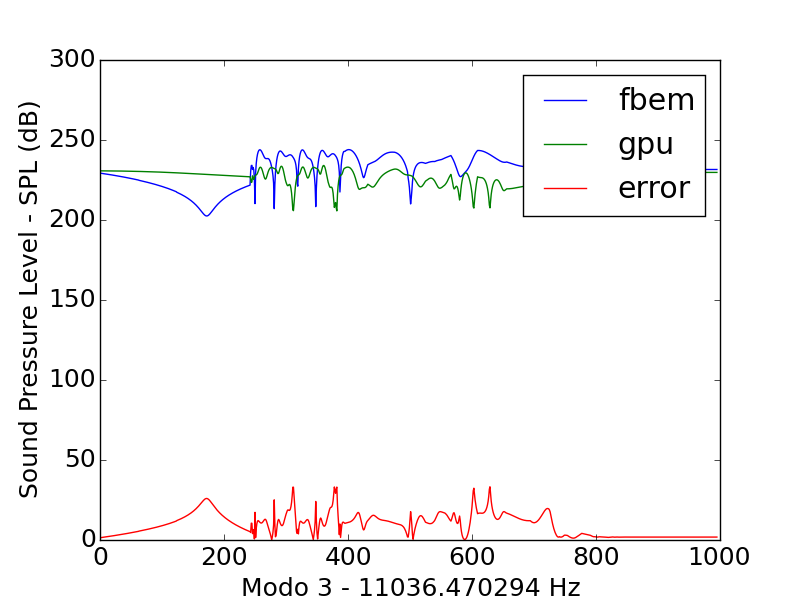
\includegraphics[width=\textwidth]{../data/transfer_test/steel_key/plots/steel_key-tfv-0_3.png}
	\label{fig:coef_key_3}
\end{subfigure}
\caption[Modos de Vibração de objetos]{Modos de Vibração de objetos. Ao topo: Modos de vibração de um prato de cerâmica. Abaixo: Modos de vibração de uma taça de vidro. Fonte: \cite{langlois2014eigenmode}}
\label{fig:coef_key}
\end{figure}

\begin{figure}[ht]
\centering
\begin{subfigure}{0.6\textwidth}
	\centering
	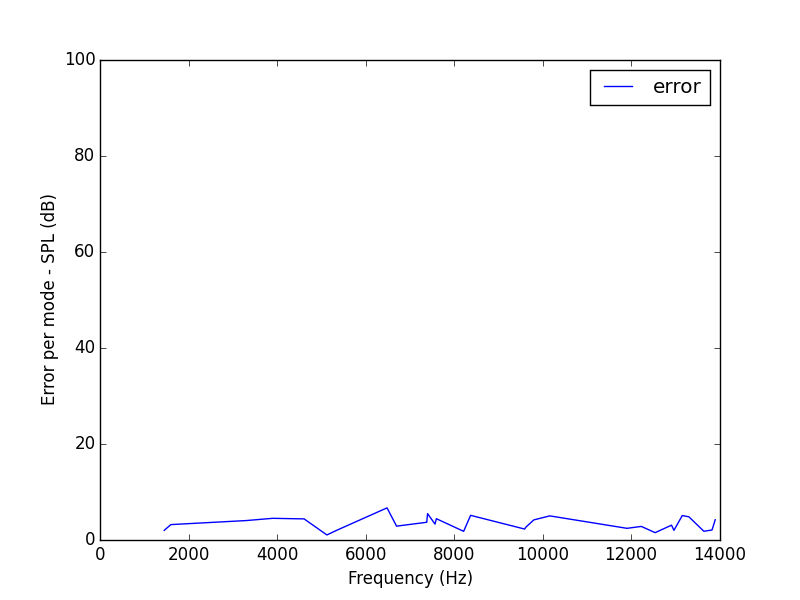
\includegraphics[width=\textwidth]{../data/transfer_test/ceramic_mug/plots/ceramic_mug_error.png}
	\label{fig:coef_mug_err}
\end{subfigure}
\begin{subfigure}{0.5\textwidth}
	\centering
	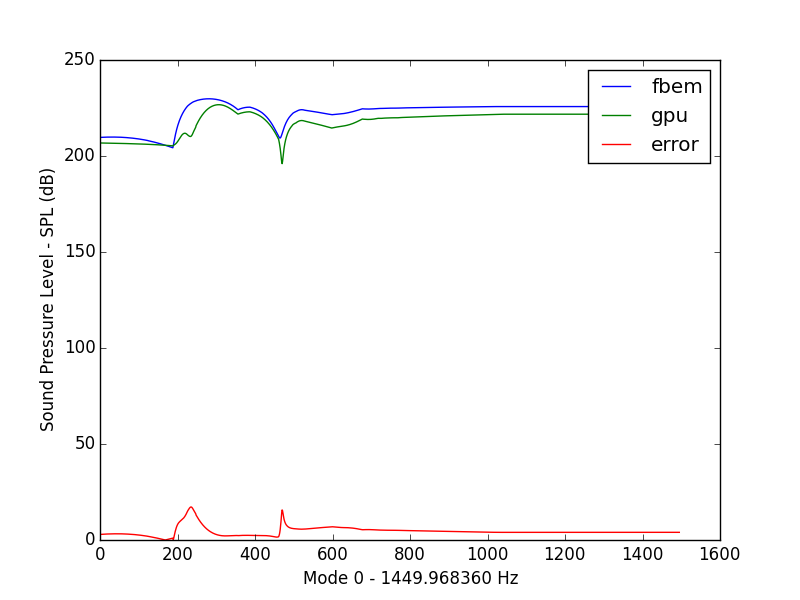
\includegraphics[width=\textwidth]{../data/transfer_test/ceramic_mug/plots/ceramic_mug-tfv-0_0.png}
	\label{fig:coef_mug_0}
\end{subfigure}%
\begin{subfigure}{0.5\textwidth}
	\centering
	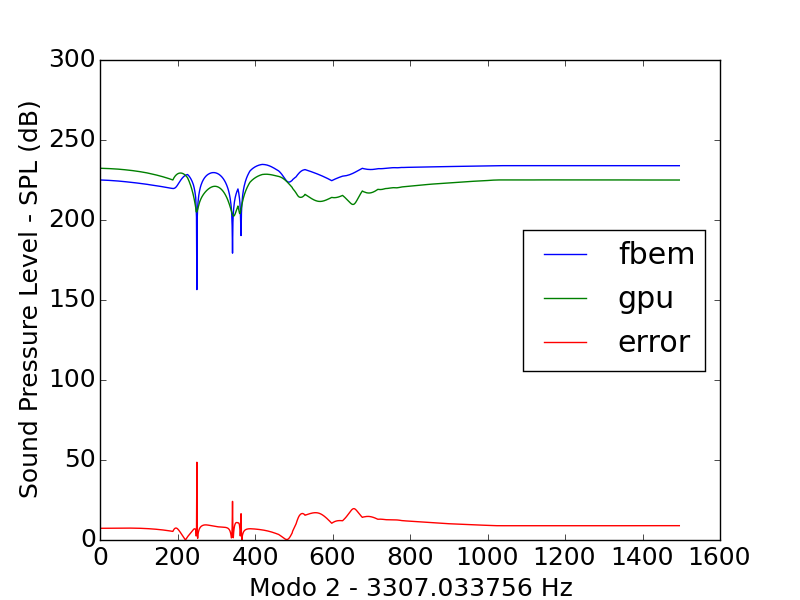
\includegraphics[width=\textwidth]{../data/transfer_test/ceramic_mug/plots/ceramic_mug-tfv-0_2.png}
	\label{fig:coef_mug_2}
\end{subfigure}
\begin{subfigure}{0.5\textwidth}
	\centering
	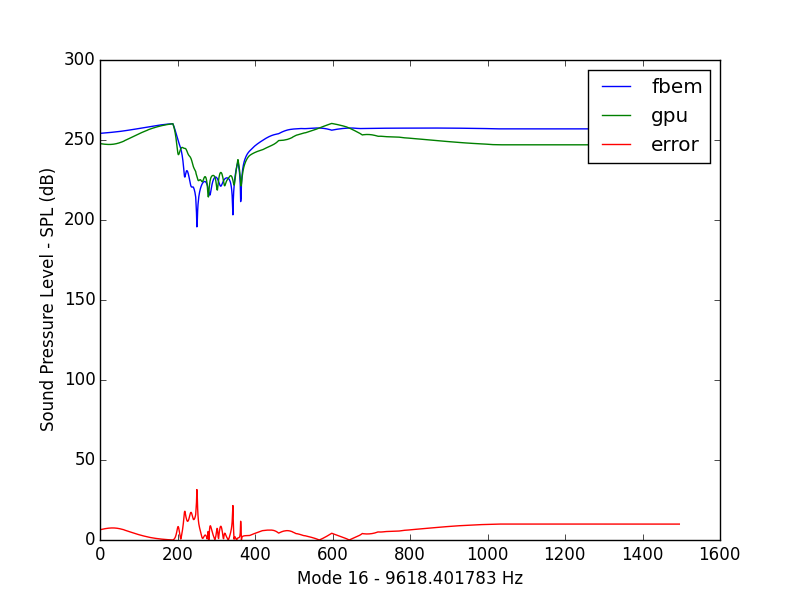
\includegraphics[width=\textwidth]{../data/transfer_test/ceramic_mug/plots/ceramic_mug-tfv-0_16.png}
	\label{fig:coef_mug_16}
\end{subfigure}%
\begin{subfigure}{0.5\textwidth}
	\centering
	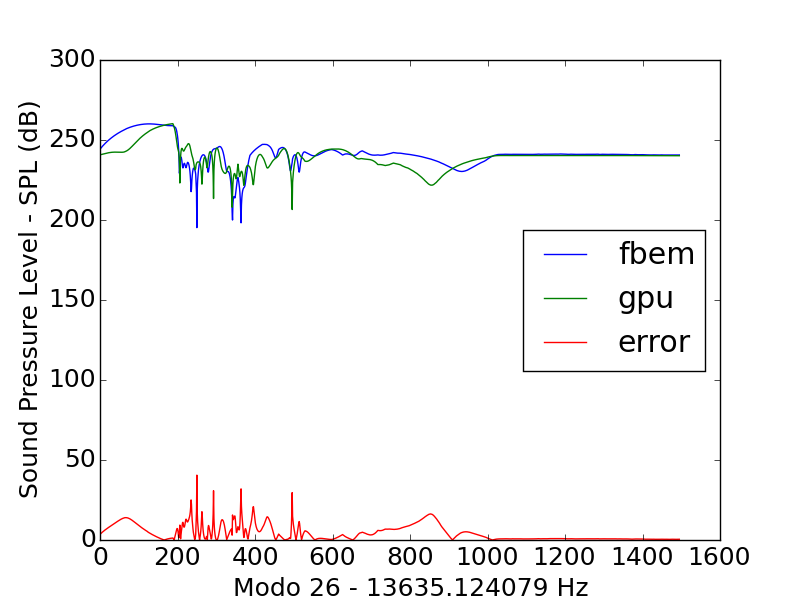
\includegraphics[width=\textwidth]{../data/transfer_test/ceramic_mug/plots/ceramic_mug-tfv-0_26.png}
	\label{fig:coef_mug_26}
\end{subfigure}
\caption[Modos de Vibração de objetos]{Modos de Vibração de objetos. Ao topo: Modos de vibração de um prato de cerâmica. Abaixo: Modos de vibração de uma taça de vidro. Fonte: \cite{langlois2014eigenmode}}
\label{fig:coef_mug}
\end{figure}

\begin{figure}[ht]
\centering
\begin{subfigure}{0.6\textwidth}
	\centering
	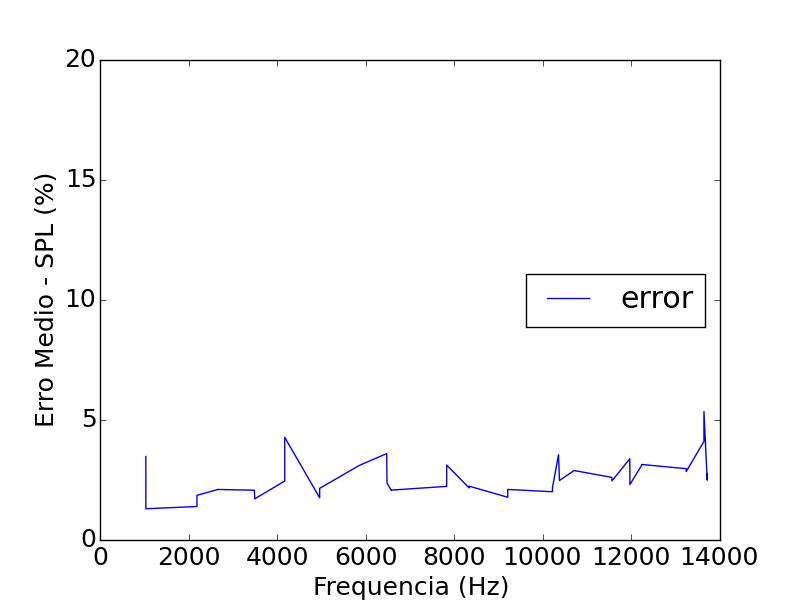
\includegraphics[width=\textwidth]{../data/transfer_test/ceramic_plate/plots/ceramic_plate_error.png}
	\label{fig:coef_plate_err}
\end{subfigure}
\begin{subfigure}{0.5\textwidth}
	\centering
	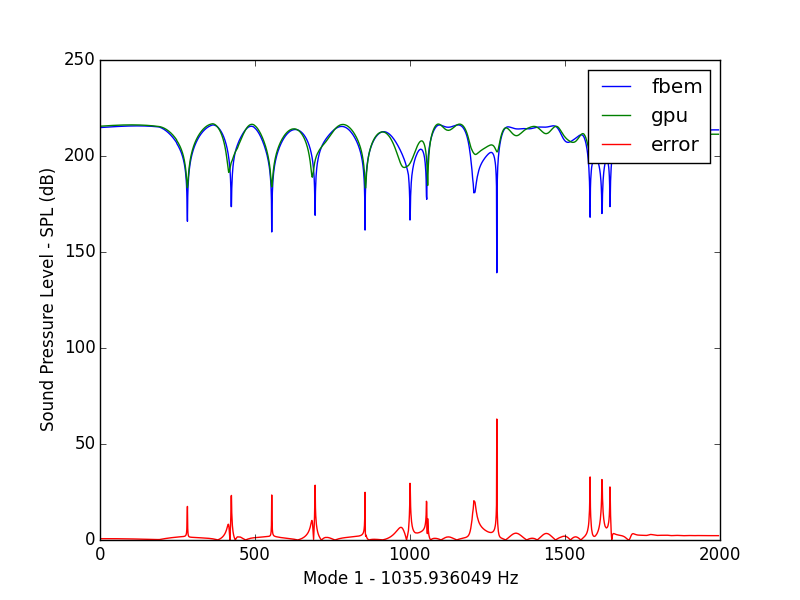
\includegraphics[width=\textwidth]{../data/transfer_test/ceramic_plate/plots/ceramic_plate-tfv-0_1.png}
	\label{fig:coef_plate_1}
\end{subfigure}%
\begin{subfigure}{0.5\textwidth}
	\centering
	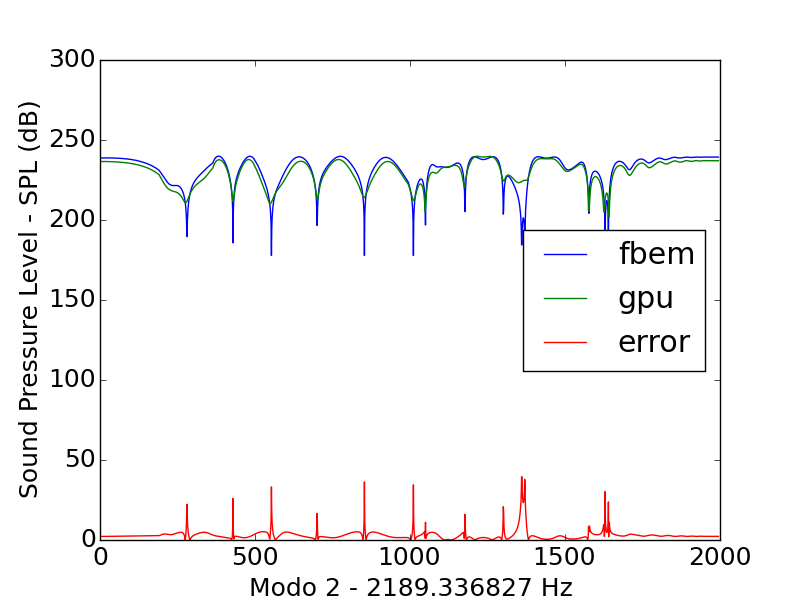
\includegraphics[width=\textwidth]{../data/transfer_test/ceramic_plate/plots/ceramic_plate-tfv-0_2.png}
	\label{fig:coef_plate_2}
\end{subfigure}
\begin{subfigure}{0.5\textwidth}
	\centering
	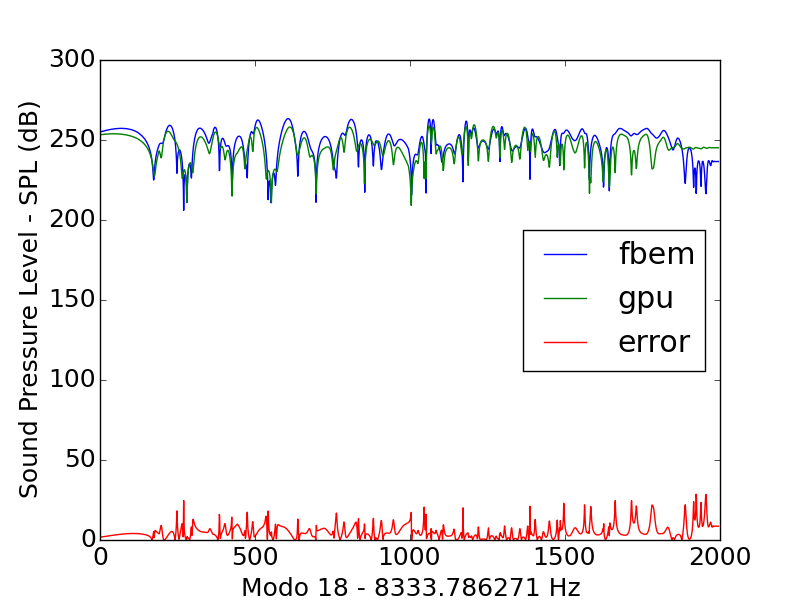
\includegraphics[width=\textwidth]{../data/transfer_test/ceramic_plate/plots/ceramic_plate-tfv-0_18.png}
	\label{fig:coef_plate_18}
\end{subfigure}%
\begin{subfigure}{0.5\textwidth}
	\centering
	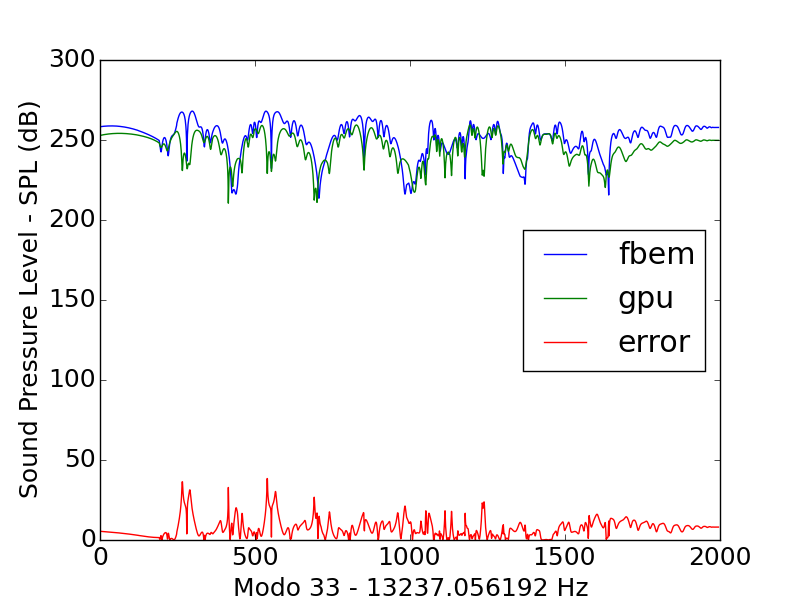
\includegraphics[width=\textwidth]{../data/transfer_test/ceramic_plate/plots/ceramic_plate-tfv-0_33.png}
	\label{fig:coef_plate_33}
\end{subfigure}
\caption[Modos de Vibração de objetos]{Modos de Vibração de objetos. Ao topo: Modos de vibração de um prato de cerâmica. Abaixo: Modos de vibração de uma taça de vidro. Fonte: \cite{langlois2014eigenmode}}
\label{fig:coef_plate}
\end{figure}


\section{Teste de Percepção}

Para testarmos a qualidade final do áudio sintetizado, geramos três cenários distintos. Para cada cenário, geramos um áudio com os coeficientes calculados pelo FastBEM e outro áudio com os coeficientes calculados com o nosso método. O restante do pipeline não foi modificado.

Um teste A/B foi feito com voluntários. Nesse teste, o voluntário assistia ambas as versões do vídeo (identificadas apenas por A ou B) e deveria responder à pergunta: ``Qual dos dois pareceu mais realista? A ou B?''. O voluntário tinha como opções: ``A'', ``B'' ou ``Não sei''. A \tabref{tab:survey_results} contém o resultado da pesquisa.

\begin{table}[ht]
\begin{center}
\begin{tabular}{c|ccccc}
Cena & Nosso Método & FastBEM & Não sei & Total\\
\hline Prato de Cerâmica & $70.5\%$ & $24\%$ & $5.5\%$ & $100\%$\\
Caneca de Cerâmica & $64.6\%$ & $24\%$ & $11.4\%$ & $100\%$\\
Prato de Cerâmica & $46.9\%$ & $20.5\%$ & $32.7\%$ & $100\%$\\
Total & & & & 254 respostas
\end{tabular}
\end{center}
\caption{Resultado dos Testes de Percepção}\label{tab:survey_results}
\end{table}



